\documentclass[a4paper]{article} 
\addtolength{\hoffset}{-2.25cm}
\addtolength{\textwidth}{4.5cm}
\addtolength{\voffset}{-3.25cm}
\addtolength{\textheight}{5cm}
\setlength{\parskip}{0pt}
\setlength{\parindent}{0in}

\usepackage{blindtext} % Package to generate dummy text
\usepackage{charter} % Use the Charter font
\usepackage[utf8]{inputenc} % Use UTF-8 encoding
\usepackage{microtype} % Slightly tweak font spacing for aesthetics
\usepackage[english]{babel} % Language hyphenation and typographical rules
\usepackage{amsthm, amsmath, amssymb, amsfonts} % Mathematical typesetting
\usepackage{float} % Improved interface for floating objects
\usepackage[final, colorlinks = true, 
linkcolor = black, 
citecolor = black]{hyperref} % For hyperlinks in the PDF
\usepackage{graphicx, multicol} % Enhanced support for graphics
\usepackage{xcolor} % Driver-independent color extensions
\usepackage{marvosym, wasysym} % More symbols
\usepackage{rotating} % Rotation tools
\usepackage{subcaption}
\usepackage{wrapfig}
\usepackage{censor} % Facilities for controlling restricted text
\newcommand{\note}[1]{\marginpar{\scriptsize \textcolor{red}{#1}}} % Enables comments in red on margin
\usepackage{bm}
\usepackage{blkarray}
\usepackage{enumitem}
\usepackage{pgfplots}
\usepackage{tikz}
\usepackage{bbm}
\usepackage[autostyle]{csquotes} 

\newcommand{\pd}[2]{\frac{\partial #1}{\partial #2}}
\newcommand{\loss}[0]{\mathcal{L}}
\newcommand{\chain}[3]{\frac{\partial #1}{\partial #2}\frac{\partial #2}{\partial #3}}
\newcommand{\eq}[1]{\begin{equation*}\begin{split}#1\end{split}\end{equation*}}
\newcommand{\TODO}[1]{\textbf{\textcolor{red}{#1}}}
\newcommand{\comment}[1]{\textit{\textcolor{blue}{Comment: #1}}}

\definecolor{green}{RGB}{0,160,0}
\definecolor{blue}{RGB}{0,0,160}
\definecolor{red}{RGB}{160,0,0}
\definecolor{orange}{RGB}{200,160,0}
\definecolor{purple}{RGB}{170,0,200}
\definecolor{cyan}{RGB}{0,200,200}
\definecolor{lightred}{RGB}{200,50,50}

\setcounter{tocdepth}{2}
% Title Page
\title{Summary Machine Learning for the Quantified Self}
\author{Phillip Lippe}


\begin{document}
\maketitle
\tableofcontents
\newpage

\section{Introduction}
\label{sec:chapter_1_2_introduction}
\subsection{Definitions}
\begin{itemize}
	\item The quantified self can be defined as:
	\blockquote{\textit{The quantified self is any individual engaged in the self-tracking of any kind of biological, physical, behavioral, or environmental information. \\The self-tracking is driven by a certain goal of the individual with a desire to act upon the collected information.}}
	\item \textbf{Augemberg} (2012): there are various types of measurements, including:
	\begin{itemize}
		\item Physical activities (movement by accelerometer, steps, etc.)
		\item Diet (calories consumed, fat, protein, etc.)
		\item Psychological states (mood, emotions, depression, etc.)
		\item Mental and cognitive traits (IQ, reaction, memory, etc.)
		\item Environmental (location, weather, etc.)
		\item Situational (time of the day, context, etc.)
		\item Social variables (influence, role in a group, etc.)
	\end{itemize} 
	\item \textbf{Choe} (2014): distinguish quantified selves into three categories based on their goal.
	\begin{itemize}
		\item Improved health (cure or manage a condition,
		execute a treatment plan, achieve a goal)
		\item Improve other aspects of life (maximize work performance, be mindful)
		\item Find new life experiences (have fun, learn new things)	
	\end{itemize}
	\item \textbf{Gimpel} (2013): identified five (non-exclusive) factors for quantified self motivation
	\begin{itemize}
		\item Self-healing (to become healthier)
		\item Self-discipline (to experience rewarding aspects of it)
		\item Self-design (to control and optimize ``yourself'', as e.g. on sport)
		\item Self-association (to be associated with the movement of QS)
		\item Self-entertainment (to experience entertainment value)
	\end{itemize}
	\item Machine Learning (automatically identifying patterns from data) is slightly different in the setting of Quantified Self because
	\begin{itemize}
		\item we have to deal with sensory noise
		\item there might be missing measurements
		\item we have temporal data (feature engineering) with irregular time points
		\item there can be an interaction with a user (advice for training/mood improvements, etc.), but we cannot try out every possibility
		\item Learn across multiple datasets/users
	\end{itemize}
	\item \comment{Most of the above definitions need to be memorized for the exam}
\end{itemize}
\subsection{Basic Terminology and Notation}
\begin{itemize}
	\item Measurement $=$ one value for an attribute recorded at a specific time point
	\item Time series $=$ series of measurements in temporal order
	\item Further notation: 
	\begin{itemize}
		\item For matrix $\bm{X}$, the columns are the different measurements like accelerometer, and rows are the time points (if dataset is temporally ordered, otherwise random list) 
	\end{itemize}
	\begin{figure}[ht!]
		\centering
		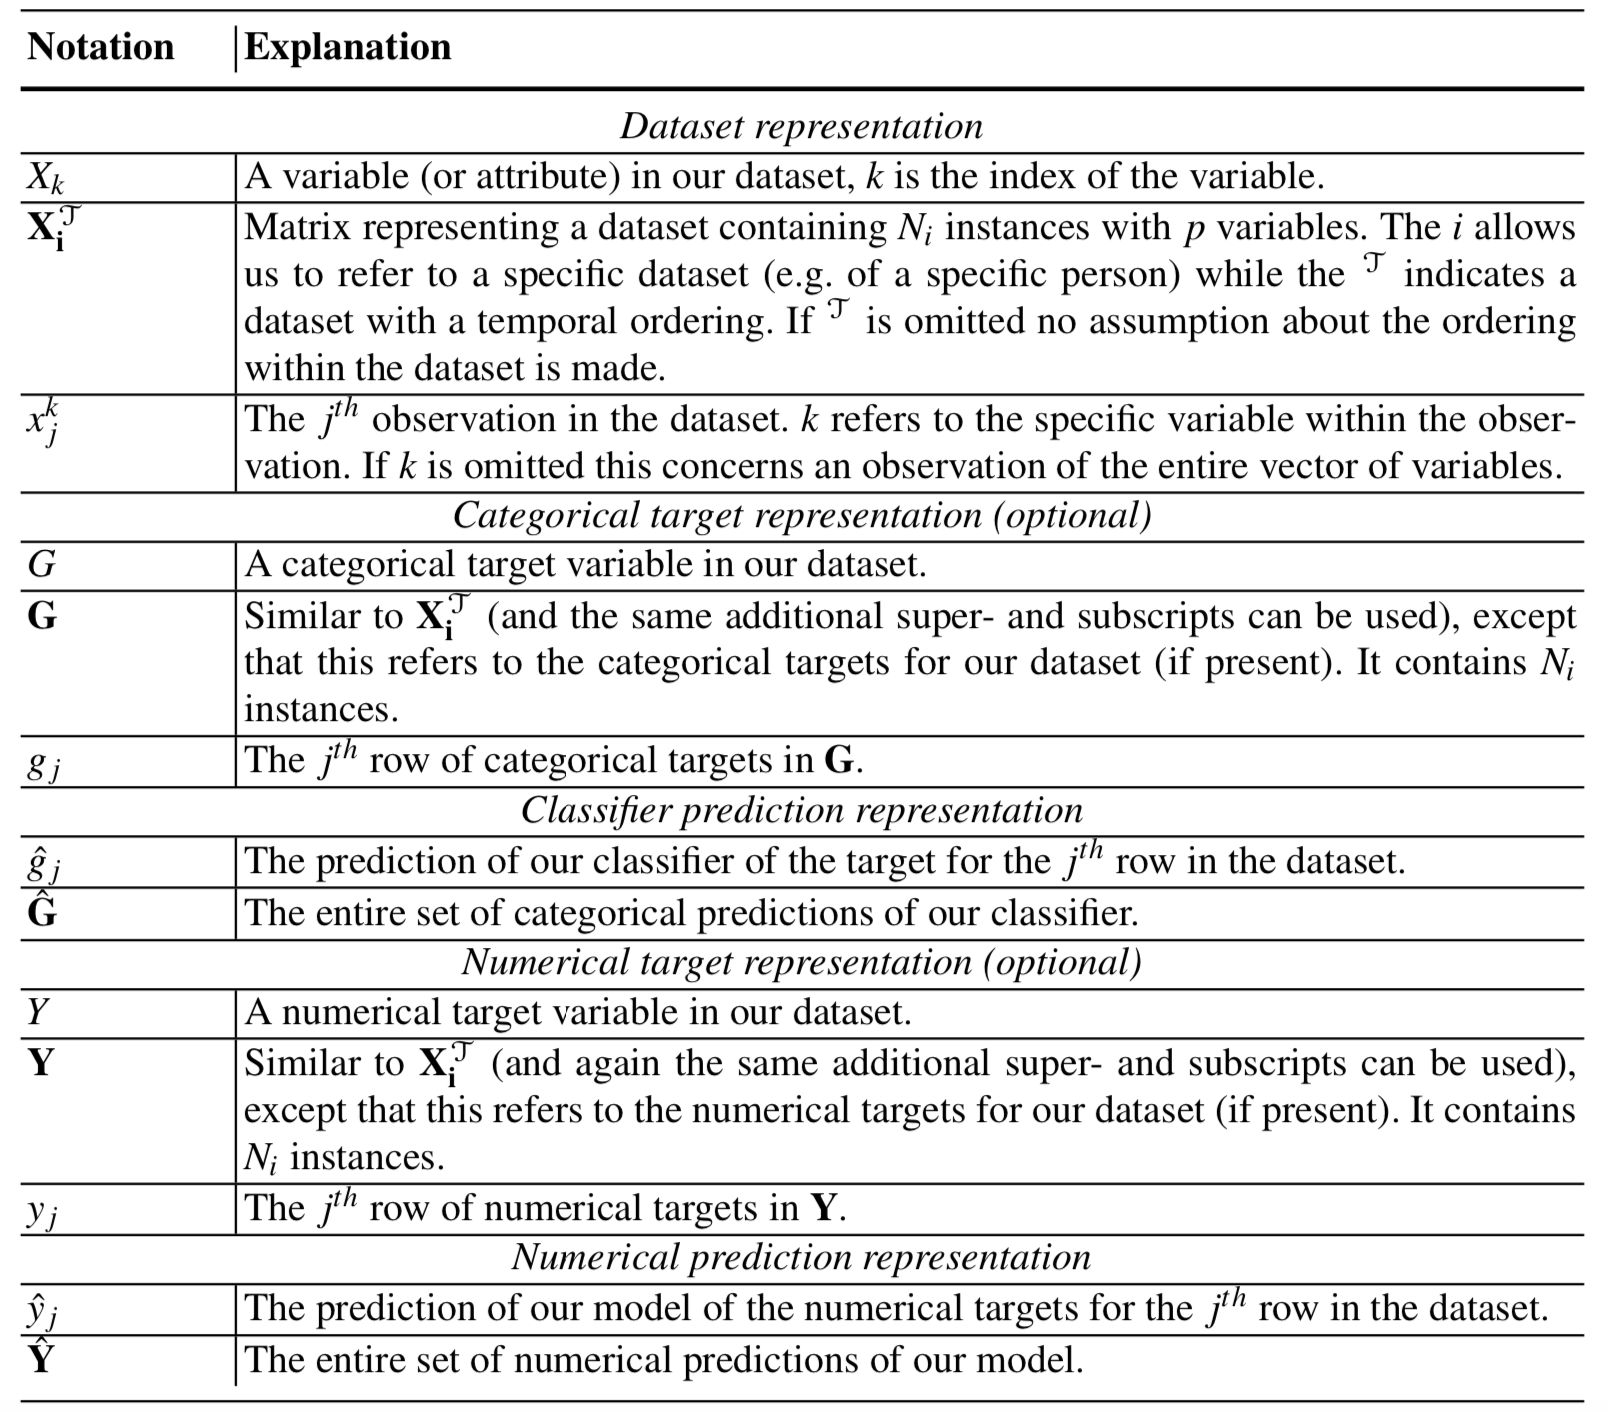
\includegraphics[width=0.4\textwidth]{figures/intro_notation.png}
		\caption{Overview of notation used in this course.}
	\end{figure}
\end{itemize}
\subsection{Basic overview of Sensory Data}
\begin{itemize}
	\item Different sensors available on mobile devices, such as:
	\begin{itemize}
		\item \textit{Accelerometer}: Measures the changes in forces upon the phone in the $x$-$y$-$z$ plane
		\item \textit{Gyroscope}: Orientation of the phone compared to
		the earth's surface
		\item \textit{Magnetometer}: Measures $x$-$y$-$z$ orientation compared to the earth's magnetic field
	\end{itemize}
	\item Transforming raw data of time series require selecting a step size $\Delta t$, and combine sensory data over this interval. See Section~\ref{sec:chapter_4_feature_engineering} for techniques
	\item A large $\Delta t$ gives (maybe too) coarse-grained data, but we have in the end a smaller dataset and lower standard deviation. The opposite is gained by a smaller $\Delta t$ (fine-grained data, but large dataset and high stddev)
\end{itemize}
\section{Handling Sensory Noise}
\label{sec:chapter_3_sensory_noise}
\subsection{Outlier Detection}
\begin{itemize}
	\item ``\textit{An outlier is an observation point that is distant from other observations}''
	\item Outliers can be caused by measurement errors, or variability of the data (e.g. very high heart rate due to pushing someone's limits)
	\item Outliers can be detected by either \textit{domain knowledge} (known in what range to expect value, e.g. heart rate should not be over 220), or without by filtering noise. We distinguish between two ways for doing so:
	\begin{itemize}
		\item \textit{Distribution-based}: assume a certain distribution of the data, and remove all points with a likelihood lower than a certain threshold
		\item \textit{Distance-based}: focus on the distance between data points, and mark those as outliers which are far apart
	\end{itemize}
	\item After detecting the outliers, we can replace them with \textit{unknown} values/value missing tag. 
\end{itemize}
\subsubsection{Distribution-based outlier detection}
\begin{itemize}
	\item \textbf{Chauvenet's criterion}: assume a normal distribution for a single attribute
	\begin{itemize}
		\item We can fit a normal distribution by calculating the mean and stddev of the data
		\item For each point, calculate the probability $P(X\leq x_{i}^{j})=\int_{-\infty}^{x_{i}^{j}} \frac{1}{\sqrt{2\pi}\sigma}e^{-\frac{(u-\mu)^2}{2\sigma^2}} \partial u$\\ (instance $i$ from $j$th attribute)
		\item A point is an outlier if:
		$$P(X\leq x_{i}^{j}) < \frac{1}{c\cdot N} \hspace{3mm}\text{or}\hspace{3mm} \left(1-P(X\leq x_{i}^{j})\right) < \frac{1}{c\cdot N}$$
		Thus, the probability of a point being an outlier decreases with the number of observations for this attribute (as the likelihood increases to observe rare values)
		\item Mostly $c=2$ is chosen.
	\end{itemize}
	\item \textbf{Mixture models}: assume the data to be described by $K$ normal distributions $p(x)=\sum_{k=1}^{K}\pi_k \mathcal{N}\left(x|\mu_k, \sigma_k\right)$
	\begin{itemize}
		\item Use EM algorithm to optimize maximum-likelihood of the data
		\item A point is considered as an outlier if it has a lower probability than a certain threshold
		\item Both threshold and number of distributions $K$ is a hyperparameter to optimize
	\end{itemize}
\end{itemize}
\subsubsection{Distance-based outlier detection}
\begin{itemize}
	\item Outlier detection based on a distance metric $d(x_{i}^{j}, x_{k}^{j})$ (as e.g. Euclidean distance) which can also be across multiple attributes
	\item \textbf{Simple distance-based approach}:
	\begin{itemize}
		\item Call two points close if they are within a distance $d_{\text{min}}$ (hyperparameter)
		\item A point $x_{i}^{j}$ is considered as an outlier if:
		$$\frac{\sum_{n=1}^{N} \mathbbm{1}\left(d(x_{i}^{j}, x_{n}^{j}) > d_{\text{min}}\right)}{N} > f_{\text{min}}$$
		Hence, we look if the number of points within the range of $d_{\text{min}}$ are at least $1-f_{\text{min}}$.
		\item Example values of hyperparameters: $d_{\text{min}}=0.1, f_{\text{min}}=0.99$
		\item Not working if we have multi-modal distribution (does not take local densities into account)
	\end{itemize}
	\item \textbf{Local outlier factor}: use local densities to determine outliers.
	\begin{itemize}
		\item Define $k_{\text{dist}}$ for point $x_{i}$ as the maximum distance in set of its $k$ closest neighbors. 
		\item The reachability distance of $x_{i}$ \textbf{from} $x$ is defined as:
		$$k_{\text{reach\_dist}}(x_i, x) = \max\left(k_{\text{dist}}(x), d(x, x_i)\right)$$
		Note that this distance is \textit{not} symmetric as it uses the $k$th nearest neighbors of a point.\\
		Furthermore, this operation is only done to reduce the influence of very close-by points. 
		\item The local reachability distance of a point is defined by:
		$$k_{\text{lrd}}\left(x_{i}\right) = \frac{\left|k_{\text{distnh}}\left(x_{i}\right)\right| }{\sum\limits_{x\in k_{\text{distnh}}\left(x_{i}\right)} k_{\text{reach\_dist}}\left(x_i, x\right)}$$
		Hence, it is high if a point is very close to others.
		\item Outlier if neighbor points have much higher local reachability points than actual point:
		$$k_{\text{lof}}\left(x_{i}\right) = \frac{\sum\limits_{x\in k_{\text{distnh}}\left(x_{i}\right)} k_{\text{lrd}}\left(x\right)}{\left|k_{\text{distnh}}\left(x_{i}\right)\right| \cdot k_{\text{lrd}}\left(x_{i}\right)}$$
	\end{itemize}
\end{itemize}
\subsection{Missing value imputation}
\begin{itemize}
	\item Due to outliers or measuring errors, we might have missing values in our dataset
	\item We can use simple methods like replace it by the mean or median of the other observed data, or also use more advanced methods that take the values of the other attributes at this observation into account, or a local time window.
	\begin{itemize}
		\item Example for the latter: \textbf{interpolation} $x_{i}^{j} = x_{i-k}^{j} + k \cdot \frac{x_{i+l}^{j} - x_{i-k}^{j}}{l+k}$
	\end{itemize}
\end{itemize}
\subsubsection{Kalman Filter}
\begin{itemize}
	\item Combine outlier detection and imputation into a single model
	\item Therefore, we keep a latent state $s_t$, for which $x_t$ are the observations in this states (Kalman filter relates $x_t$ and $s_t$)
	\item The next value of a state is defined as: $$s_t = F_t s_{t-1} + B_t u_t + w_t$$ where $u_t$ is a control input state (as e.g. sending a message), $w_t$ is white noise, and $F_t$ and $B_t$ are learned matrices
	\item The measurements associated with $s_t$ can be predicted by: $$x_t = H_t s_t + v_t$$ where $v_t$ is again white noise.
	\item We can predict the next state (without noise) by $\hat{s}_{t|t-1} = F_t \hat{s}_{t-1|t-1} + B_t u_t$
	\item The error at time $t$ compared to the observations $x_t$ is then $e_t = x_t - H^T \hat{s}_{t|t-1}$
	\begin{itemize}
		\item If we observe (after training/modeling) a high error, we can assume a value to be an outlier, and replace it with the prediction of the Kalman Filter.
	\end{itemize}
	\item Given this error, we can update our prediction accordingly: $\hat{s}_{t|t} = \hat{s}_{t|t-1} + K_t e_t$ where $K_t$ takes the expected prediction error into account (based on the white noise $w_t$ and $v_t$)
	% \item Next, we can estimate our prediction error of $\hat{s}_{t|t-1}$ by $P_{t|t-1}=\mathbb{E}\left[\left(s_t - \hat{s}_{t|t-1}\right)\left(s_t - \hat{s}_{t|t-1}\right)^T\right]$
\end{itemize}
\subsection{Transforming the Data}
\begin{itemize}
	\item Transform data to extract most useful data, and get rid of remaining noise
	\item Different approaches can be used
	\item \textbf{Lowpass filter}: filter out high-frequent noise
	\begin{itemize}
		\item We assume that our signal has a certain periodicity, but we are only interested in certain parts of the frequency band (noise is mostly very high-frequent)
		\item The low-pass filter can remove those by weighting each periodicity by its frequency:
		$$|G(f)|^2 = \frac{1}{1+\left(f/f_c\right)^{2n}}$$
		with $|G(f)|$ as the magnitude, $f_c$ is the cutoff frequency (magnitude halved), and $n$ the order of the filter
	\end{itemize}
	\item \textbf{Principal Component Analysis}: find components that explain most of the variance in the data
	\begin{itemize}
		\item Select number of components based on the explained variance. Other, low-variance components are removed to reduce noise 
		\item Problem: we loose insight in the data because the components are not easily interpretable anymore
	\end{itemize}
\end{itemize}
\section{Feature Engineering}
\label{sec:chapter_4_feature_engineering}
\begin{itemize}
	\item Create useful features from temporal data
\end{itemize}
\subsection{Time Domain}
\begin{itemize}
	\item Summarize values of a certain attributes in a window size of $\lambda$ steps before. If we would take the time steps $t$ and $t-1$ into account, our value for $\lambda$ is $1$
	\item Note that we cannot compute any values for the time steps $t=1,..,\lambda$.
\end{itemize}
\subsubsection{Numerical}
\begin{itemize}
	\item Aggregate values by mean, min, max, stddev, etc. (including current time step)
	\item We could also use coefficient between first and last value interpolation (gradient of attribute)
\end{itemize}
\subsubsection{Categorical}
\begin{itemize}
	\item Generate patterns of occurrences of categorical values. We distinguish between successive \texttt{(b)} and co-occurring \texttt{(c)} actions/classes. Example patterns:
	\begin{itemize}
		\item Activity level = high \texttt{(c)} Activity = running
		\item Activity = running \texttt{(b)} Activity = running
	\end{itemize}
	\item If we have a window size of $\lambda$, we just see if there is any time step within $t-\lambda, ..., t-1, t$ where the activities are co-occuring \texttt{(c)}, or there is one activity happening (arbitrary number of time steps) before another \texttt{(b)}.
	\item We can find important patterns by determining the support of such. This is important as the number of patterns exponentially increases with the number of categories/attributes, and only frequent patterns are interesting.
	\item The support of a pattern is defined as the proportion of the processed time steps at which this pattern would occur.
	\item The algorithm for finding such patterns starts with single attribute patterns, and extends only those which have sufficient support. In the end, we add all patterns (including the single-attribute) with enough support.
	\begin{figure}[ht!]
		\centering
		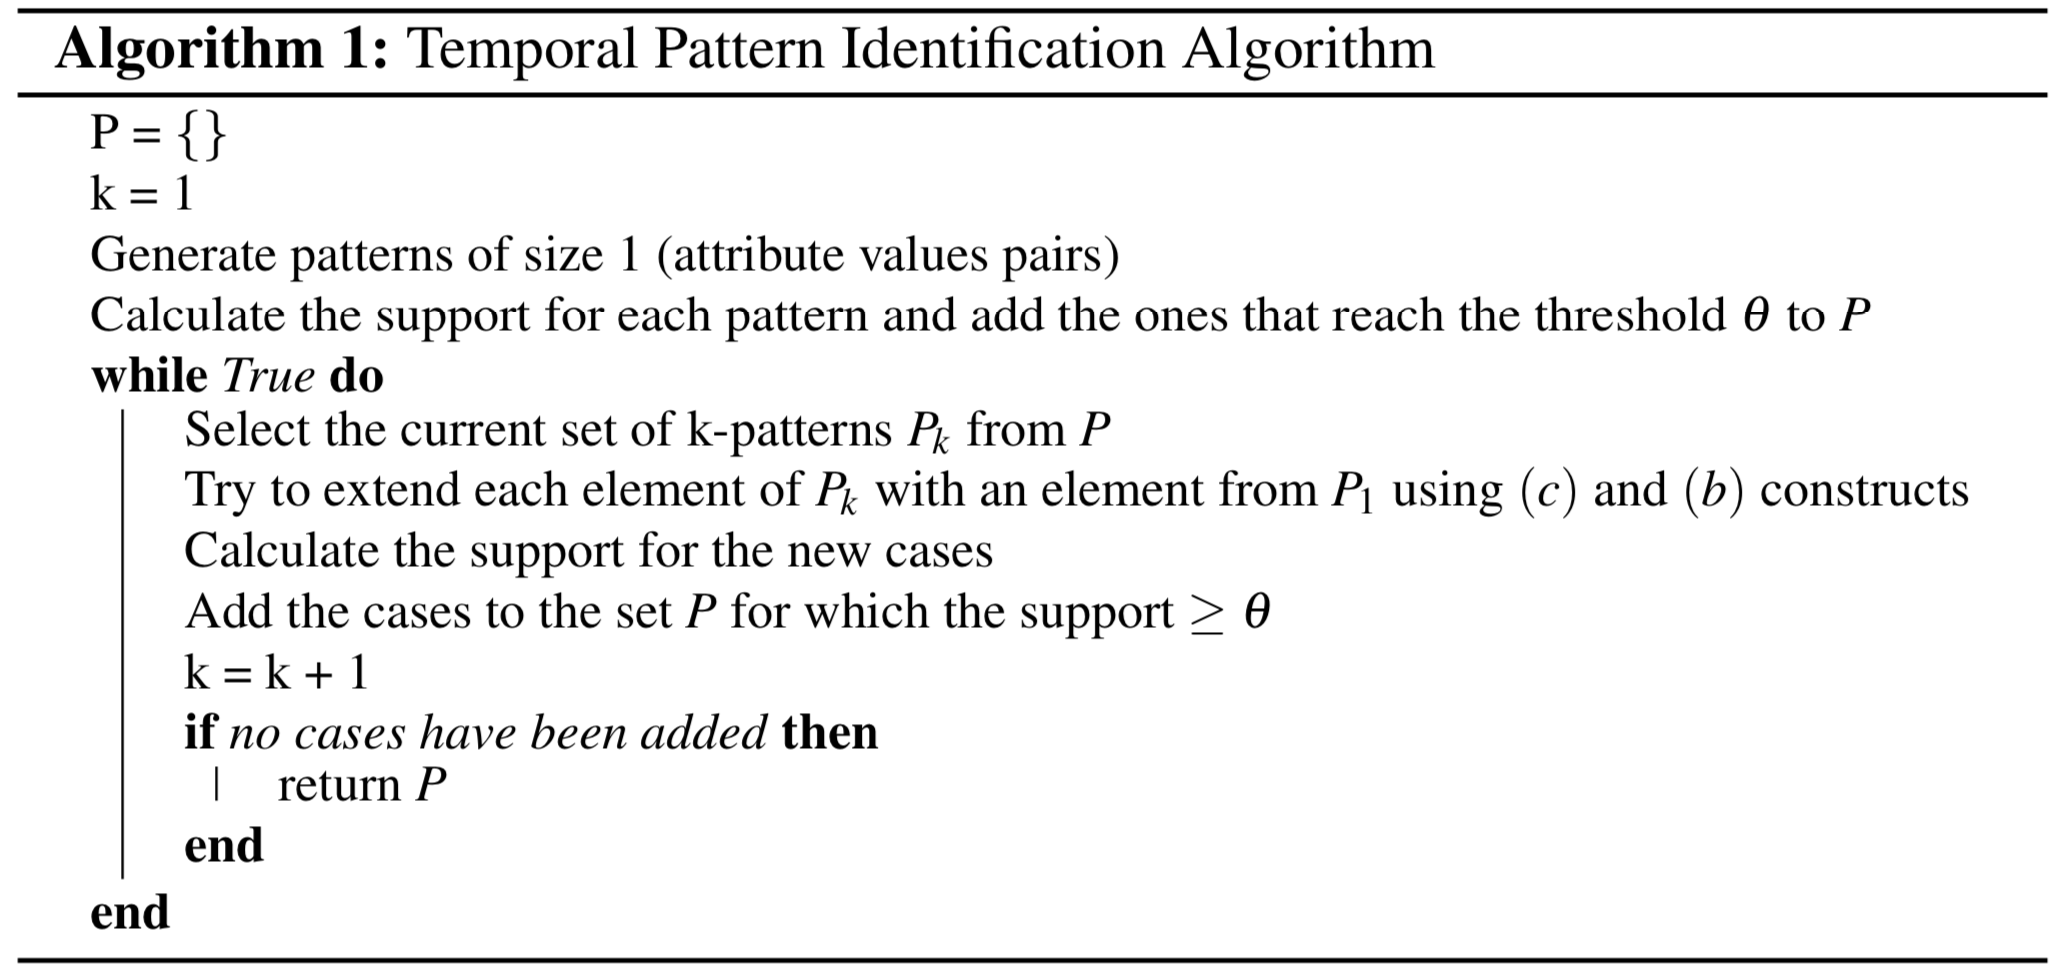
\includegraphics[width=0.5\textwidth]{figures/chapter_4_pattern_identification.png}
		\caption{Pattern identification algorithm}
	\end{figure}
\end{itemize}
\subsubsection{Mixed data}
\begin{itemize}
	\item We can also combine numerical and categorical attributes for features
	\item Hereby, we create categories from numerical data by looking at them \textbf{qualitatively} (greetings from QR). For example, we can define ranges like low, medium and high, or look at the trend/gradients as \textit{increasing} or \textit{decreasing}
	\item Afterwards, we can apply the categorical approach on those
\end{itemize}
\subsection{Frequency Domain}
\begin{itemize}
	\item Apply Fourier transformation on data within a window of $\lambda$ (plus the current time point $t$) to extract periodicity of the data
	\item Assume a base frequency of $f_0 = \frac{2\pi}{\lambda+1}$ (or $f_0 = \frac{N_{\text{sec}}}{\lambda+1}$ in seconds) which is the lowest frequency with a complete sinusoid in it. 
	\item We look at all the frequencies $\left\{0\cdot f_0, 1\cdot f_0, ..., \lambda \cdot f_0\right\}$ and determine the corresponding amplitudes
	\item Our features can be:
	\begin{itemize}
		\item Frequency with highest amplitude
		\item Frequency-weighted signal average $\frac{\sum_{k=0}^{\lambda} a_{t-\lambda}^{t}(k) \cdot f(k)}{\sum_{k=0}^{\lambda} a_{t-\lambda}^{t}(k)}$
		\item \textit{Power Spectrum Entropy}: Amount of information in the signal
		$$x\_pse = - \sum_{k=0}^{\lambda} p_{t-\lambda}^{t}(k) \ln p_{t-\lambda}^{t}(k), \hspace{3mm}\text{with}\hspace{2mm} p_{t-\lambda}^{t}(k) = \frac{|a_{t-\lambda}^{t}(k)|^2}{\sum_{i=0}^{\lambda} |a_{t-\lambda}^{t}(i)|^2}$$
	\end{itemize}
\end{itemize}
\subsection{Unstructured data}
\begin{itemize}
	\item How to handle non-temporal/unstructured data like text, audio, images, etc.
	\item Here we focus on text. The standard pipeline contains for steps:
	\begin{itemize}
		\item \textit{Tokenization}: split sentence into smallest parts 
		\item \textit{Lower case}: put all words to lower case to have no difference in such
		\item \textit{Stemming}: reduce words to their stem to remove all small variations (like tense, etc.)
		\item \textit{Stop word removal}: remove known, uninformative stop words 
	\end{itemize}
	\begin{figure}[ht!]
		\centering
		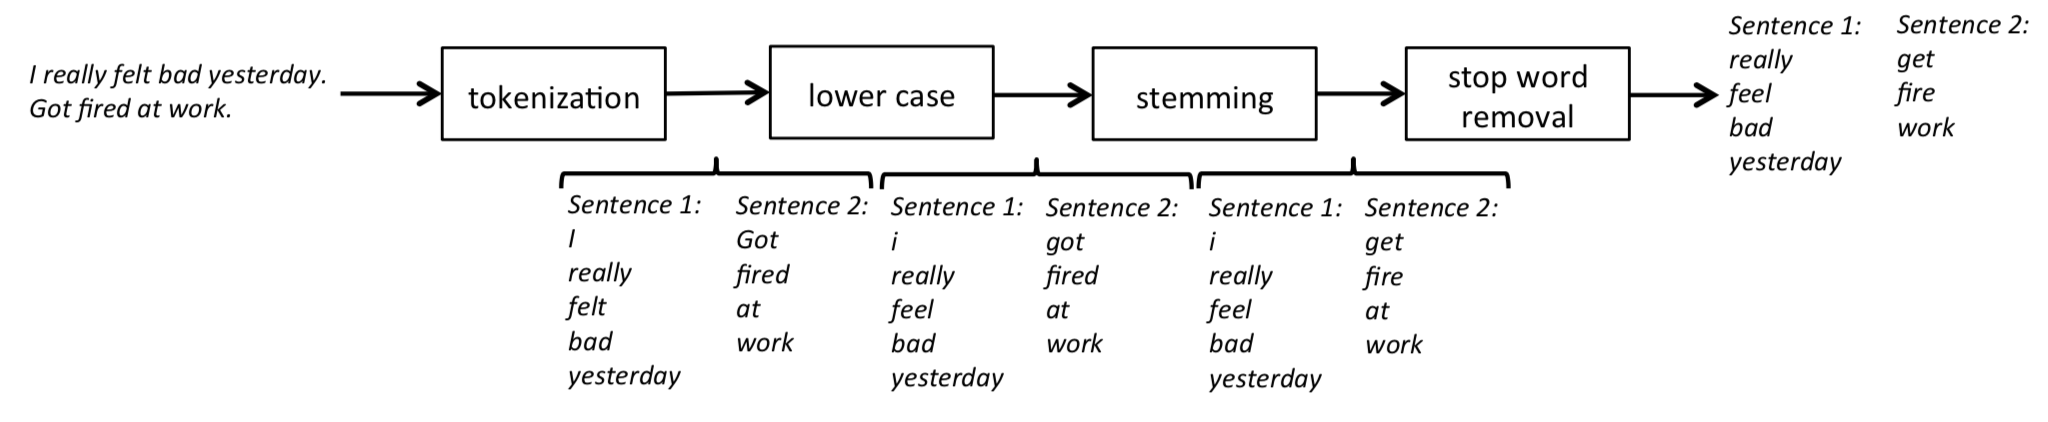
\includegraphics[width=0.5\textwidth]{figures/chapter_4_text_pipeline.png}
		\caption{Pipeline of text processing}
	\end{figure}
	\item Three approaches in general
	\begin{itemize}
		\item \textbf{Bag of words}: count occurrences of n-gram within text. These counts are the features for the text
		\item \textbf{TF-IDF}: BoW does not take ``uniqueness'' of word into account. Thus, TF-IDF takes occurrences of a word in a text and in the whole corpus into account
		\item \textbf{Topic modeling}: assume that any text is a combination of $k$ topics. Perform LDA to get these topics, and topic distribution of text is its features.
	\end{itemize}
\end{itemize}
\section{Clustering}
\begin{itemize}
	\item Using the features engineered before to cluster instances
	\item Two different learning setups
	\begin{itemize}
		\item \textit{Per instance}: cluster data points/instances of quantified selfs. If multiple quantified selfs are available, we concatenate the datasets.
		\item \textit{Per person}: cluster different quantified selfs. Here, we consider all recorded instances of a person as a single data point, and we compare datasets/persons and cluster them. 
	\end{itemize}
\end{itemize}
\subsection{Distance Metrics}
\begin{itemize}
	\item We need different distance metrics per scenario
	\item We have to distinguish between feature-level and dataset-level
\end{itemize}
\subsubsection{Feature-level distance metrics}
\begin{itemize}
	\item For \textit{numerical} features, we can use the minkowski distance $\left(\sum_k \left|x_i^k - x_j^k\right|^q\right)^{1/q}$ which subsumes the Euclidean and Manhatten ($q=1$). However, we need to consider the scaling of the features (assumed to be equal)
	\item For \textit{categorical} features, we can use the Gower's similarity
	\begin{itemize}
		\item For binary attributes (called \textit{dichotomous}) $s(x_i^k, x_j^k)=1$ if $x_i^k$ and $x_j^k$ are present (i.e. are 1), else 0
		\item For categorical, we have $s(x_i^k, x_j^k)=\mathbbm{1}(x_i^k = x_j^k)$
		\item For numerical values in a range $R$, the Gower's similarity is $s(x_i^k, x_j^k)=1 - \frac{|x_i^k - x_j^k|}{R}$
		\item Similarity over multiple attributes is the mean of them
		\item Note that this is a similarity and not a distance (correlated by $\text{Similarity}\sim1/\text{Distance}$)
	\end{itemize}
\end{itemize}
\subsubsection{Dataset-level distance metrics}
\begin{itemize}
	\item We have to distinguish between datasets with and without temporal ordering
	\item \textbf{Non-temporal personal level distance metrics}: three different approaches possible
	\begin{enumerate}
		\item Summarize values per attribute over the entire dataset into a single number, as e.g. take the mean, min, max, stddev, etc. On these, we can use the same distance metrics as before
		\item Estimate parameters of a distribution that describes the dataset, such as a normal distribution with $\mathcal{N}(\mu, \sigma^2)$. On the parameters $\mu, \sigma^2$ we can apply the same distance metrics as before
		\item Compare the distributions of values for an attribute with a statistical test, such as the Kolmogorov Smirnov test. The distance metric would be $1-p$ where $p$ is the $p$-value returned by the test.
	\end{enumerate}
	\item \textbf{Temporal personal level distance metrics}: again, three different approaches
	\begin{enumerate}
		\item \textit{Feature-based}: extract features from the two time series, such as those from Section~\ref{sec:chapter_4_feature_engineering} (time and frequency domain).
		\item \textit{Model-based}: we try to fit a model on the two time series, and use those parameters to compare them. For example, we could use dynamical systems or similar
		\item \textit{Raw-data based} uses a distance per point.
		\begin{itemize}
			\item For example, it can assume a equal number of points in both datasets, and just takes e.g. the Euclidean Distance per time point
			\item Alternatively, we can also take a possible lag into account (shifted dataset). Then we compute the cross correlation coefficient $ccc(\tau, x_{qs_i}^{l}, x_{qs_j}^{l})=\sum_{k=-\infty}^{\infty} x_{k, qs_i}^{l} \cdot x_{k+\tau, qs_j}^{l}$. 
			\item Optimize $\tau$ by $\arg\min_{\tau} \sum_{k=1}^{p} \frac{1}{ccc\left(\tau, x_{qs_i}^{l}, x_{qs_j}^{l}\right)}$. Note that we have a single $\tau$ for all attributes
			\item \textbf{Dynamic Time Warping}: make best pairs of instances in the sequence to find minimum distance. Allows different frequencies of activities
			\begin{itemize}
				\item Two conditions for pairing: \\
				\textit{Monoticity condition}: time order has to be preserved. We cannot go ``back'' in time\\
				\textit{Boundary condition}: the first and last point must be aligned of the two time series
				\item Algorithm similar to finding shortest path in a graph.
				\begin{figure}[ht!]
					\centering
					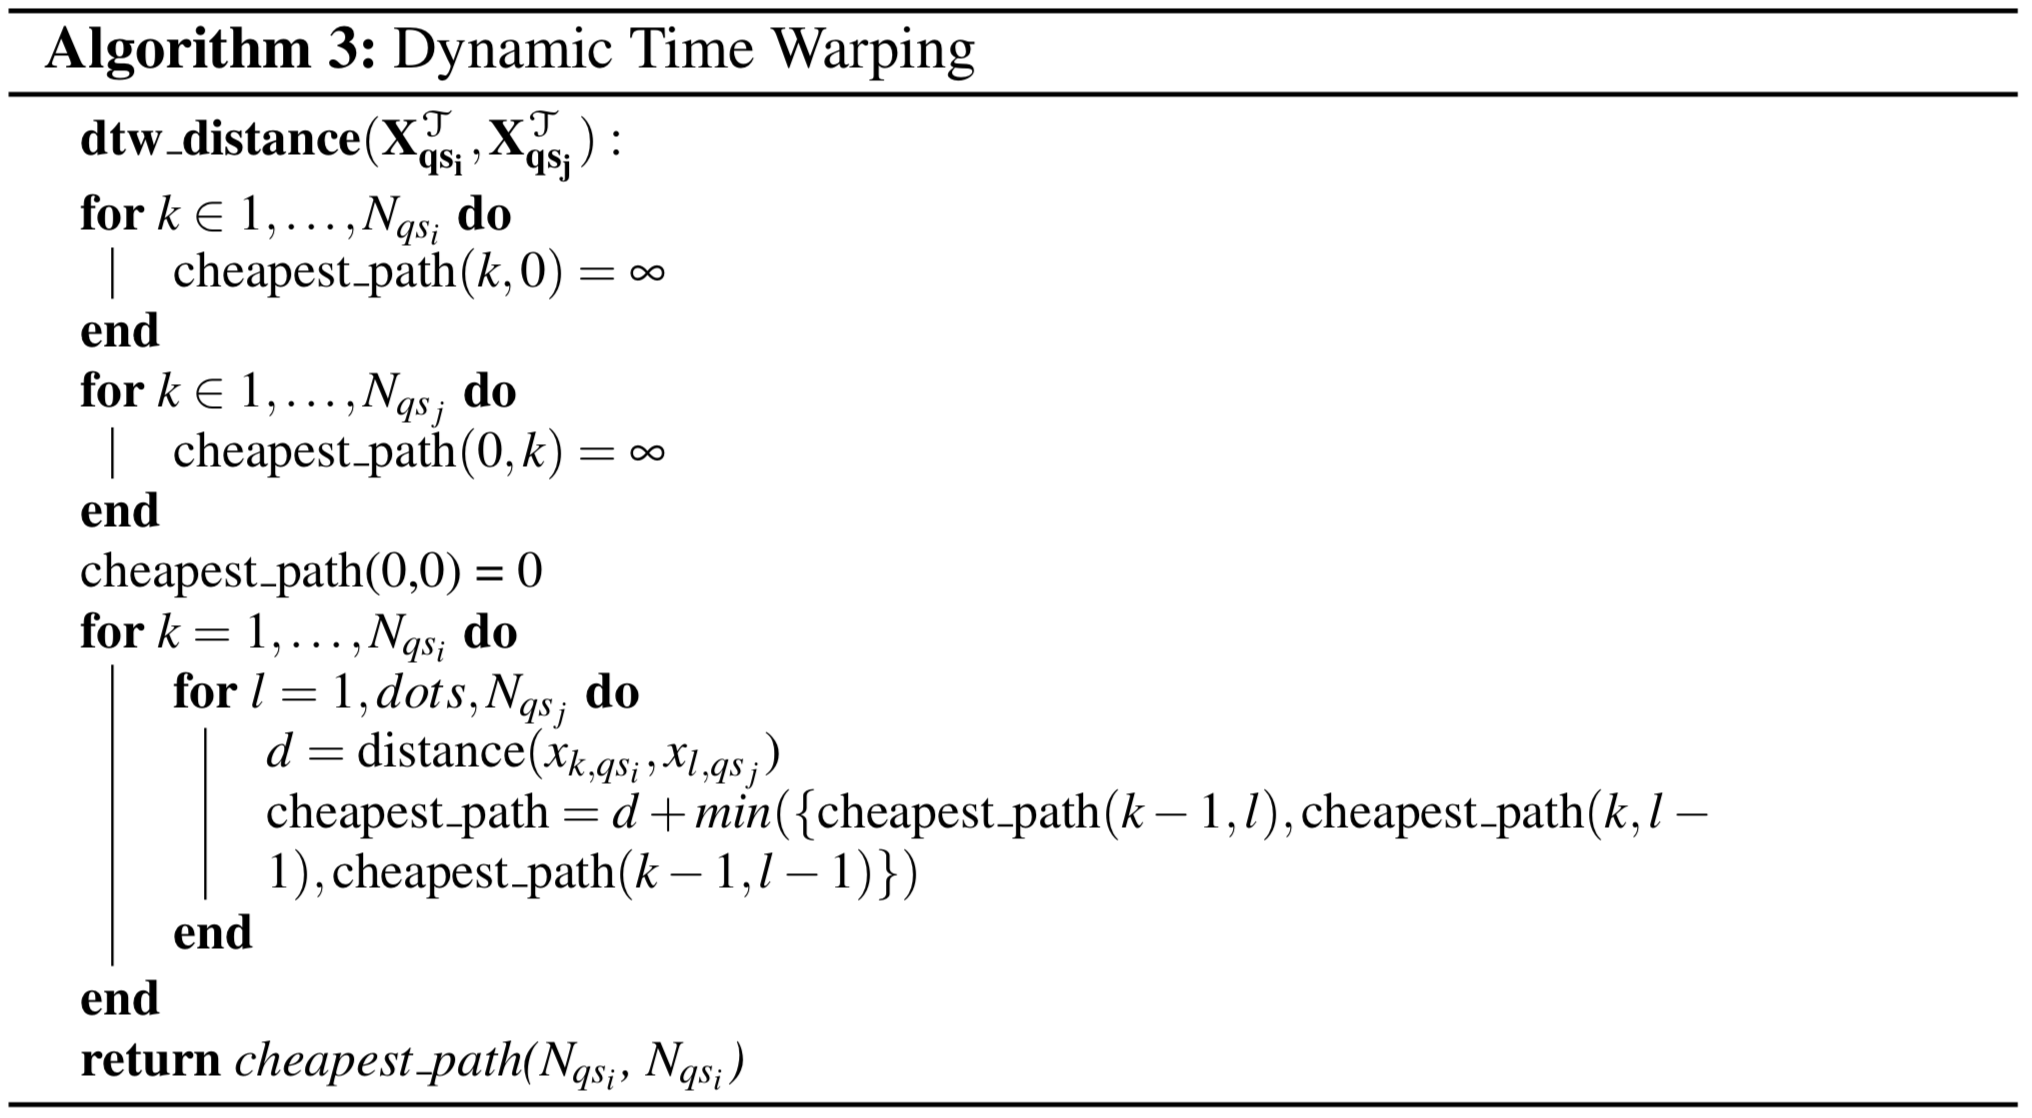
\includegraphics[width=0.5\textwidth]{figures/chapter_5_dynamic_time_warping.png}
					\caption{Algorithm of dynamic time warping}
				\end{figure}
				\item The drawbacks of this methods are that it is computational expensive ($\mathcal{O}(N\cdot M)$), and that the distance metric might not always be the best fit (i.e. should it be allowed to align the first point of sequence 1 with the last point of sequence 2?)
				\item \comment{For this algorithm, it helps more to practice it several times instead of writing it down in all details.}
			\end{itemize}
		\end{itemize} 
	\end{enumerate}
\end{itemize}
\subsection{Clustering approaches}
\begin{itemize}
	\item Overview of different clustering approaches
	\item \textbf{K-means}: define $k$ cluster means. A point is assigned to the cluster to which mean it is the closest. Means are updated by the assigned points.
	\begin{itemize}
		\item Using Silhoutte score to select best $k$/determine whether a clustering is good:
		\begin{equation*}
			\begin{split}
				\text{silhoutte} = \frac{\sum_{i=1}^{N}\frac{b(x_i) - a(x_i)}{\max(a(x_i), b(x_i)}}{N}\hspace{3mm} & \text{where}\hspace{2mm} a(x_i)=\frac{\sum_{\forall x_j \in C_l} d(x_i, x_j)}{|C_l|} \hspace{3mm} \text{(} x_i\in C_l\text{)}\\
				& \hspace{2mm}\text{and} \hspace{4mm} b(x_i) = \min_{C_m \neq C_l}\frac{\sum_{\forall x_j \in C_m} d(x_i, x_j)}{|C_m|}
			\end{split}
		\end{equation*}
		In text, the silhoutte score compares the average distance of a point with others within a cluster ($a(x_i)$) with the distance of points with the next closest cluster ($b(x_i)$). The larger the score, the better (between$[-1,1]$)
	\end{itemize}
	\item \textbf{K-medoids}: very similar to $k$-means, but we use actual points as cluster centers instead of artificial ones
	\begin{itemize}
		\item Choose new cluster means as the point with the minimum distance to all other points in the cluster
		\item More suitable if certain points in search space might not make sense
		\item For example, k-medoids is known to work better for person-level clustering
	\end{itemize}
\end{itemize}
\subsubsection{Hierarchical clustering}
\begin{itemize}
	\item Perform clustering in an iterative approach
	\item \textbf{Divisive clustering}: start with one cluster with all points in it, and in each step, perform one split
	\begin{itemize}
		\item Define the dissimilarity of a point to all other points in a cluster as the average distance $$\text{dissimilarity}(x_i, C)=\frac{\sum_{x_j\neq x_i \in C} \text{distance}(x_i, x_j)}{|C|}$$
		\item When creating a new cluster $C'$, we add the most dissimilar points (in order of dissimilarity) until a point is more dissimilar to the points in $C'$ than points in $C$. 
		\item If we have multiple clusters, we choose the cluster to split which has the greatest distance between any points in the cluster
	\end{itemize}
	\item \textbf{Agglomerative clustering}: start with all points in separate clusters, and merge them step by step. Merge decision can be based on different criteria (equal to distance metric between clusters):
	\begin{itemize}
		\item \textit{Single linkage}: merge the two clusters with the minimum distance between any two points
		$$d_{SL}(C_k, C_l) = \min\limits_{x_i \in C_k, x_j \in C_l} \text{distance}(x_i, x_j)$$
		\item \textit{Complete linkage}: merge the two clusters where the maximum distance between any two points is minimal
		$$d_{SL}(C_k, C_l) = \max\limits_{x_i \in C_k, x_j \in C_l} \text{distance}(x_i, x_j)$$
		\item \textit{Group average}: merge the two clusters with the average distance between all points is minimal
		$$d_{SL}(C_k, C_l) = \frac{\sum\limits_{x_i \in C_k, x_j \in C_l} \text{distance}(x_i, x_j)}{|C_k|\cdot |C_l|}$$
		\item \textit{Ward's criterion}: merge the two clusters where the increase of standard deviation by the combined cluster is minimal
		$$d_{SL}(C_k, C_l) = \sigma^2_{C_k \cup C_l} - \left(\sigma^2_{C_l} + \sigma^2_{C_k}\right)$$
	\end{itemize}
\end{itemize}
\subsubsection{Subspace clustering}
\begin{itemize}
	\item The problem of standard clustering algorithms for a huge number of features is that the distance between two points get uninformative (small distance in all features compared to big difference in only one feature). Hence, the clusters get less meaningful as well
	\item Better approach is therefore to look at subspaces in the feature space.
	\item Pseudo algorithm:
	\begin{enumerate}
		\item For all features, define intervals of the feature space. This leads to units $u={u_1, ..., u_p}$ where $u_i(l)$ is the lower-bound for attribute $i$ in this unit, and $u_h(l)$ the upper bound respectively. Note that units do not require to cover all features, but can look at subspaces only (same to setting lower bound to $-\infty$ and upper to $\infty$). 
		\item Determine selectivity of a unit as proportion of points in them. We call a unit ``dense'' if it contains more points/higher proportion than a certain threshold (hyperparameter).
		\item Units are connected to a cluster if they 
		\begin{itemize}
			\item share a common face which is defined as having the lower bound equals to an upper bound of another unit (or other way round), and the same upper and lower bound for all other attributes. 
			\item or when they share a unit to which they both have a common face.
		\end{itemize}
	\end{enumerate}
	\item In the end, we strive to find dense units using a combination of attributes to form clusters
	\item To reduce number of attributes, we can start to make units with a single attribute, and add more attributes iteratively based on some \textit{fancy} algorithm. After having found the units, we can create the clusters
\end{itemize}
\section{Supervised Learning}
\begin{itemize}
	\item The perspective on supervised learning in this course is summarized in Figure~\ref{fig:chapter_6_supervised_learning}
	\begin{figure}[ht!]
		\centering
		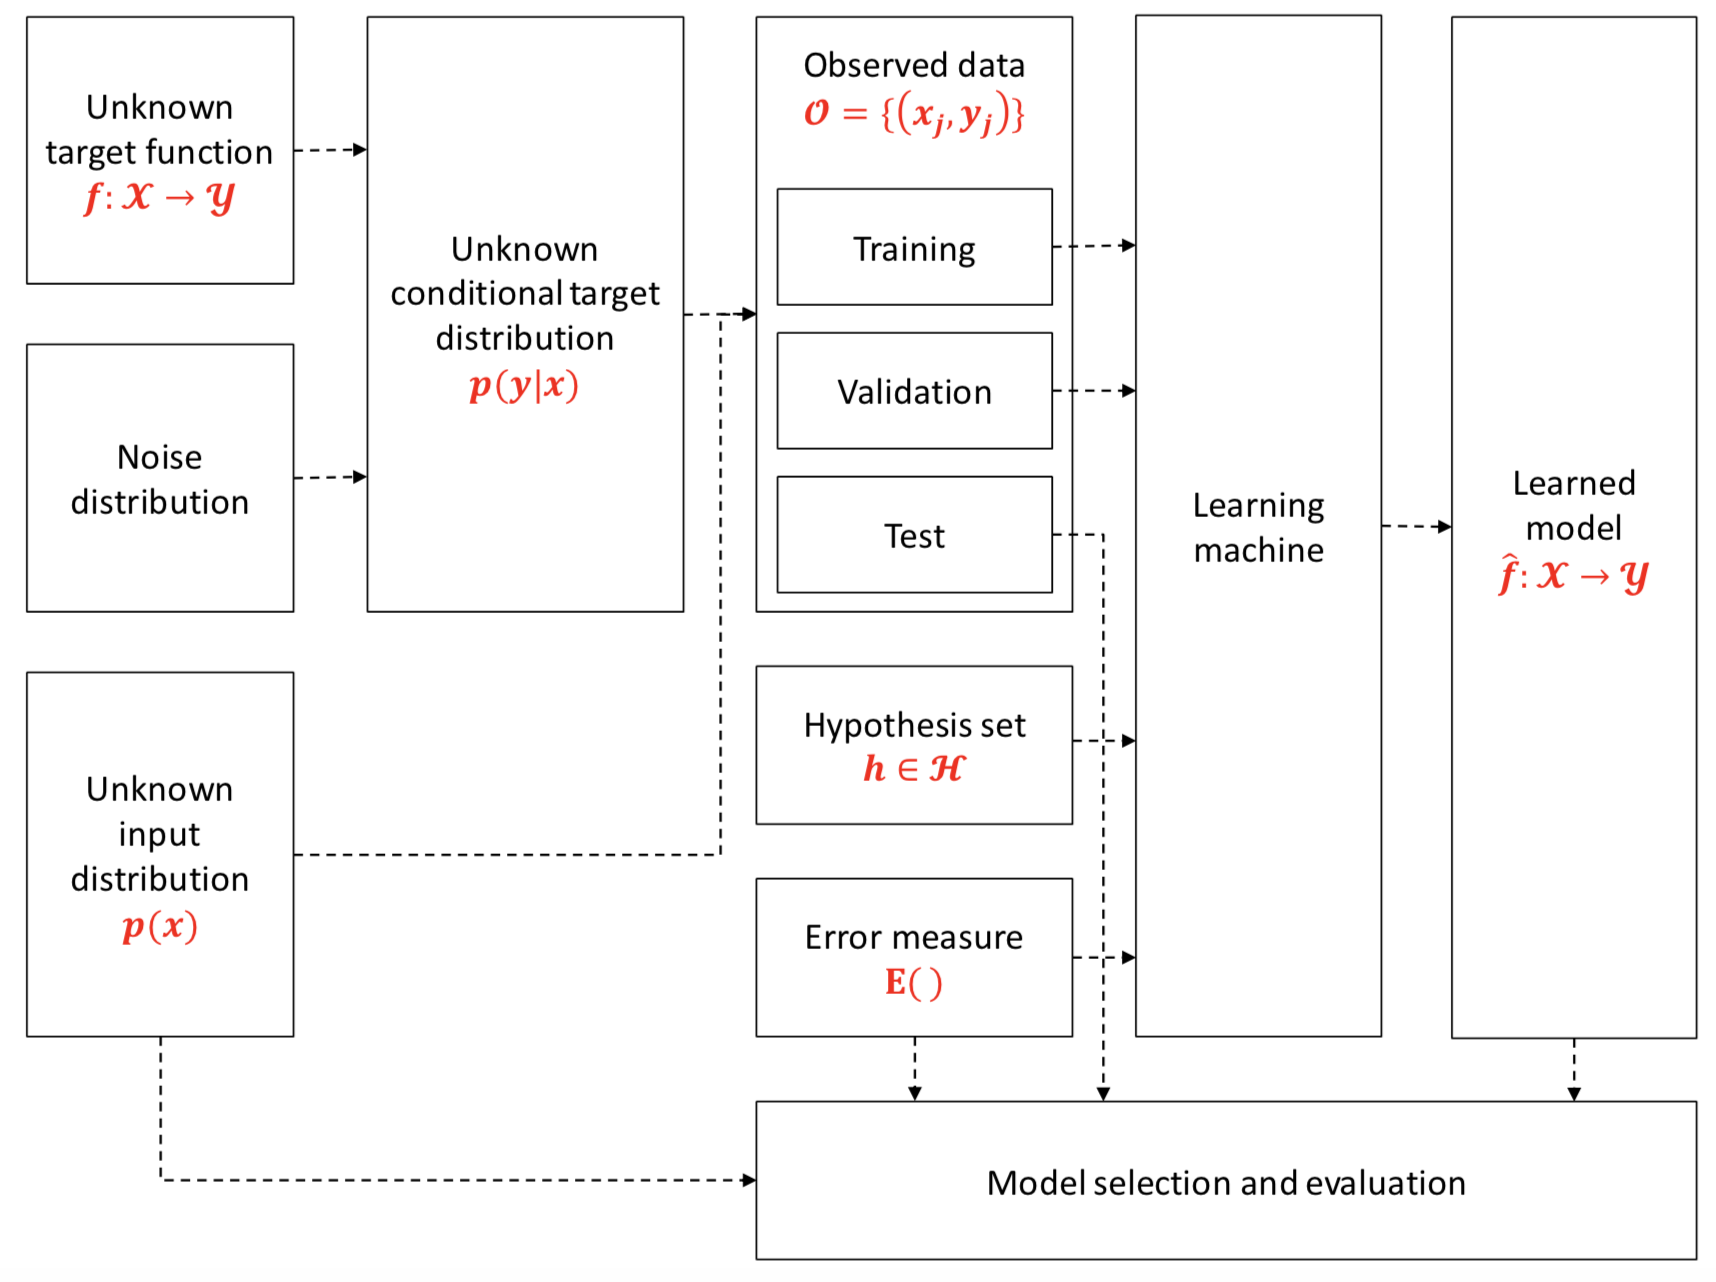
\includegraphics[width=0.5\textwidth]{figures/chapter_6_supervised_learning_overview.png}
		\caption{Overview of supervised learning framework}
		\label{fig:chapter_6_supervised_learning}
	\end{figure}
	\item Discussion of error measuring
	\begin{itemize}
		\item \textit{Risk} $E(h,f)$ describes the distance between our hypothesis $h$ and the target function $f$
		\item \textit{Loss} is the point-wise risk $e(h(x),f(x))$
		\item Given the evidence $p(x)$, we can determine the risk by $E(h,f)=\int e(h(x), f(x)) p(x) dx$
		\item However, this integral can (usually) not be computed, and only approximated by Monte-Carlo integration. 
		\item For definitions of $e$, we can use metrics like F1 or accuracy (classification), or MSE etc. (regression)
		\item The in-sample error is the average loss over all training points $E_{in}(h)=\frac{1}{N}\sum_{(x,y) \in \mathcal{O}_{\text{train}}} e(y, h(x))$
		\item The out-of-sample error accordingly for points not in the training set:\\
		$E_{out}(h)=\int_{\mathcal{X}\setminus \mathcal{O}_{\text{train}}} e(h(x), f(x)) p(x) dx$
	\end{itemize}
	\item We select the model with the lowest in-sample error, but need to be careful with overfitting
\end{itemize}
\subsection{PAC Learnability and VC dimensionality}
\begin{itemize}
	\item ``Probably approximately correct learning''
	% \item A hypothesis set is PAC learnable if a learning algorithm exists that can minimize the generalization error to $|E_{out}(\hat{f}) - E_{in}(\hat{f})| < \epsilon$ with a probability of $1-\delta$
	\item A hypothesis set is PAC learnable when it can be shown that given any value of $\delta$, $\epsilon$ there is an $N$ (number of samples) where with probability $1-\delta$ the difference between the in-sample and out-of-sample error is less than $\epsilon$. 
	\item \textit{Probably}: $1-\delta$, \textit{Approximate correct}: $|E_{out}(\hat{f}) - E_{in}(\hat{f})| < \epsilon$ 
	\item For a finite set of $M$ hypotheses, we determine it by:
	$$E_{out}(\hat{f}) \leq E_{in}(\hat{f}) + \sqrt{\frac{1}{2N}\log \frac{2M}{\delta}}$$
	Hence, every finite set of hypotheses is PAC learnable, and we can calculate the expected error given number of samples $N$, hypothesis set size $M$, and probability $\delta$
	\item For infinite set of hypotheses, we can look at VC dimensionality
	\begin{itemize}
		\item We say that a set of input vectors $X$ is shattered by a hypothesis set $\mathcal{H}$ if it can represent all possible labeling
		\item The VC dimension of $\mathcal{H}$ is an $X$ with the highest cardinality $D$. Note that not all possible point sets of cardinality $D$ must be shattered by $\mathcal{H}$. It is sufficient if it is true for at least one. 
		\item Example for a perceptron:
		\begin{figure}[ht!]
			\centering
			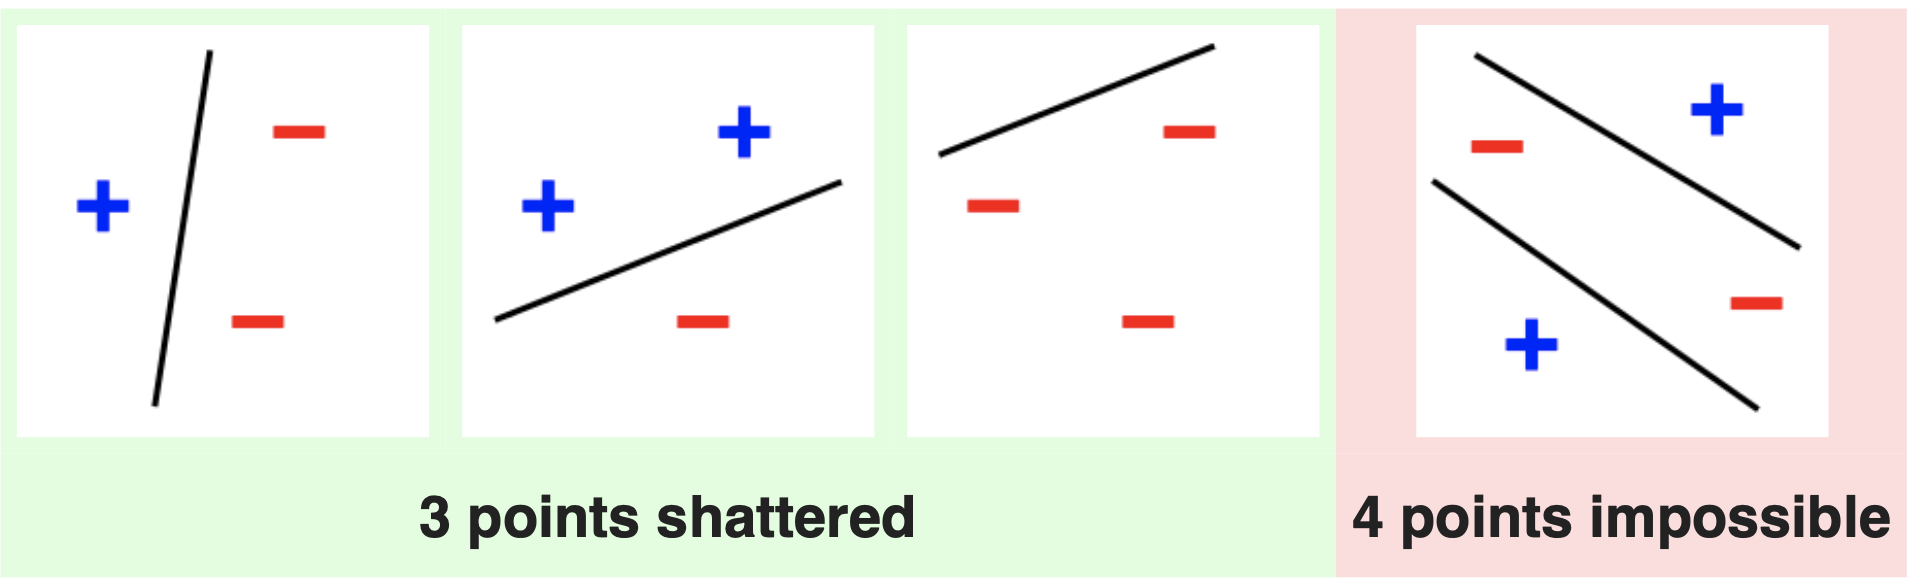
\includegraphics[width=0.3\textwidth]{figures/chapter_6_VC_dimensions.png}
		\end{figure}
	
		The VC dimension of a perceptron in 2 dimensions is $3$, because there exists no set of 4 points that can be shattered (i.e. for which we can learn any labeling)
		\item If the hypothesis set can represent any labeling for an arbitrary large set $X$, it has a VC dimension of $\infty$
		\item Important finding: all hypothesis set with a finite VC-dimension are PAC learnable
		\item We can 
	\end{itemize}
	\item Some implications from this study
	\begin{itemize}
		\item Given a few training samples, it is easy to get a low in-sample error. But with increasing number of samples, the out-of-sample error decreases
		\item In addition, for a fixed $N$, we can study the influence of more complex hypotheses and find the best compromise
		\item  
	\end{itemize}
\end{itemize}
\section{Predictive Modeling without Notion of Time}
\begin{itemize}
	\item Any predictor that does not explicitly take time into account (except the temporal features from time/frequency domain etc.)
	\item Different learning setups possible
	\begin{itemize}
		\item \textit{Individual}: train and test on a single user
		\item \textit{Population - unknown user}: train on a set of users, test on a different set of users
		\item \textit{Population - unseen data}: train on a set of users, test on the same users but different data
	\end{itemize}
\end{itemize}
\subsection{Preventing overfitting}
\begin{itemize}
	\item One big issue in the context of QS is that algorithms can easily overfit. This can be due to the big amount of features, the noise contained in them, and the usually small datasets we have
	\item \textbf{Feature selection}
	\begin{itemize}
		\item To prevent the models to overfit on not useful features, we can reduce the number of features to the essential ones
		\item \textit{Forward selection}: start with empty set, and iteratively add most predictive feature. At every iteration, we need to run a model on the previously added features plus any of the other features left. Stop when accuracy does not improve significantly anymore
		\item \textit{Backward selection}: start with all features, and iteratively remove the least predictive feature. Similar to forward selection, just doing the whole algorithm reversed.
	\end{itemize}
	\item \textbf{Regularization}: add a term to the error function to punish more for more complex models. Examples include L1/L2 regularization for NN, points per leaf for decision trees, etc.
\end{itemize}
\section{Predictive Modeling with Notion of Time}
\subsection{Time Series}
\begin{itemize}
	\item Understanding the periodicity and trends in data in the time domain. Can be used for forecasting or control (e.g. how can we influence the trend)
	\item Is build up by three components:
	\begin{itemize}
		\item \textit{Seasonality/Periodicity}: any periodic/repeating pattern over any frequency (e.g. seconds, hours or days)
		\item \textit{Trend}: how the mean evolves over time
		\item \textit{Irregular variations}: noise, everything left after we remove periodicity and trend
	\end{itemize}
	\item \textbf{Stationarity}: assumption/requirement for many algorithms applied on time series
	\begin{itemize}
		\item In general, stationarity means that the statistical properties of a process generating a time series do not change over time.
		\item We call a time series stationary if trends and periodicity are removed (mean is constant), and the variance of the remaining irregular variations is constant over time
		\item Additionally, the lagged auto correlation should be constant over time/lags $\lambda$ and close to $0$:
		$$r_{\lambda} = \frac{\sum\limits_{t=1}^{N-\lambda} (x_t - \bar{x}) (x_{t+\lambda} - \bar{x})}{\sum\limits_{t=1}^{N}(x_t - \bar{x})^2}$$
		It can provides clues of underlying pattern in the data, which should not be the case for stationary ones.
		\item If a time series is not stationary, we can mostly transform it to one by removing trend, periodicity, and try to stabilize the variance
	\end{itemize}
\end{itemize}
\subsubsection{Filtering and Smoothing}
\begin{itemize}
	\item To determine the trend of a signal, one of the simplest approaches is filtering and/or smoothing
	\item Simplest filtering is for a window size of $\pm q$ (creates a new, filtered time series):
	$$z_t = \sum\limits_{r=-q}^{q} a_r x_{t+r}$$
	\item \textbf{Differencing}
	\begin{itemize}
		\item For removing a trend, the most effective technique is differencing (or gradient filter): $z_t = x_t - x_{t-1} = \nabla x_t$. As we expect the trend to be low-frequent, the gradient is therefore small. % Periodicity is not influenced by this filter (differentiating $\sin$ just shifts it in time). % Not 100% true because if we have \sin(0.1*x), we get 0.1 * \cos(0.1 * x). Hence, 10 times smaller
		\item We can also apply this operator multiple times, leading to a $d$-th order differencing ($\nabla^d x_t$). For $d=2$, we get $z_t = \nabla^2 x_t = x_t - 2x_{t-1}+x_{t-2}$. A $d$-th order differencing can remove trends than can be approximated by a polynomial of order $d$ or lower.
		\item Drawback of differencing is that the variance of the remaining time series increases. Can be improved by using a better approximation of trend than $x_{t-1}$, as for example a exponential filtered signal $e_{t} = \sum\limits_{r=-q}^{0} \frac{\alpha(1 - \alpha)^{|r|}}{2 - \alpha} x_{t+r}$ (with e.g. $\alpha=0.05$), and use that for the differencing: $z_t = x_t - e_{t}$
		\item Still, we have to be careful as we might remove low-frequent periodicity as well ($\partial \sin(0.1\cdot x)/\partial x = 0.1 \cdot \cos(0.1 \cdot x)$ $\Rightarrow$ dampen signal by factor of 10). 
		\item If we would want to remove periodicity, we could apply the differencing operator not on two adjacent points, but two points that are moved by 1 period as the difference between those is expected to be zero (note that we need to know/estimate the frequency for that)
	\end{itemize}
\end{itemize}
\subsubsection{ARIMA}
\begin{itemize}
	\item ``Autoregressive Integrated Moving Average Model''
	\item We try to estimate a model that describes the empirical data well and can be used to forecast/predict new values
	\item For this, we learn/determine a mapping of time point $t$ to probability distribution $P_t$
	\item In ARIMA, we assume $P_t$ to be modeled by a combination of a autoregressive process (AR), and a moving average (MA) over white noise $W_t$:
	$$P_t = \underbrace{\phi_1 P_{t-1} + ... \phi_p P_{t-p} + W_t}_{\text{Autoregressive process}} + \underbrace{\theta_1 W_{t-1} + ... \theta_q W_{t-q}}_{\text{Moving Average}}$$
	Note that an AR can be expressed by an infinite MA, and the other way round. But to reduce the number of parameters, both concepts are used here.
	\item To remove the drifts of mean (trend), we apply differencing of order $d$ on $P_t$ ($V_t = \nabla^d P_t$). 
	\item Optimization of parameters
	\begin{itemize}
		\item For $p$ we can look at the autocorrelation between $x_t$ and $x_{t-p}$ to find patterns
		\item For other parameters, gridsearch with objective function as the fit to the data we have
	\end{itemize}
	\item Note that ARIMA does not take seasonality/periodicity into account. Hence, we either have to add it externally, remove it beforehand or model it as well (ARIMAX)
\end{itemize}
\subsection{Recurrent Neural Networks}
\begin{itemize}
	\item Unfolding for gradient calculation
	\item \textbf{Echo State Networks}: ``cheap'' RNNs without backprop through time
	\begin{itemize}
		\item Three weight matrices:
		\begin{itemize}
			\item $\bm{W}^{\textbf{in}}$: are the weights from the input layer to the memory (or here also called \textit{reservoir}). 
			\item $\bm{W}$: are the weights over time steps (or internally in the reservoir).
			\item $\bm{W}^{\textbf{out}}$: specify the weights from the reservoir to the output
		\end{itemize}
		\item $\bm{W}^{\textbf{in}}$ and $\bm{W}$ are randomly initialized and \textbf{fixed} during training ,while $\bm{W}^{\textbf{out}}$ is learned (either by SGD or pseudo inverse)
		\item Initialization of $\bm{W}$ need to satisfy the \textit{Echo State property} which state that the effect of a previous state should gradually decrease over time (prevent exploding values)
		\item We can ensure this by randomly initializing a matrix, dividing by its spectral radius and (optionally) scale it down even further.
		\item There are different initialization heuristics to optimize this process, but all underly the \textit{No Free Lunch} theorem (optimizing for one use case will make it worse for others)
	\end{itemize}
\end{itemize}
\subsection{Dynamical Systems}
\begin{itemize}
	\item Build domain knowledge-based models that cover temporal relationships between attributes by the meas of differential equations. Furthermore, they assume a numerical state. Very simple model for velocity:
	$$y_{vel}(t) = y_{vel}(t-1) + \gamma_1 \cdot y_{acc}(t)$$
	\item Models still contain parameters (as $\gamma_1$ above) that can/need to be tuned
	\item \textbf{Parameter optimization}: three main approaches
	\begin{itemize}
		\item \textit{Simulated Annealing}: similar to an EA with a population size of 1. 
		\begin{itemize}
			\item We have a single solution which we randomly initialize first. At each iteration, we take a random step, and compare the difference in score. 
			\item If the new point is better than the old one, we replace it. Otherwise, we replace it with a probability based on the distance between the scores, and the number of steps we have already taken. 
			\item Note that the probability decreases with number of steps. Thus, we switch from exploration in the first iterations to exploitation in the last.
		\end{itemize}
		\item \textit{Genetic Algorithms}: 
		\begin{itemize}
			\item We represent parameter values as a bit string (arbitrary number of bits per parameter, all together concatenated into one genotype), and initialize a couple of them in our population 
			\item At each iteration, we choose a set of parents from our population (based on fitness value), and perform crossover as well as mutation on the children
			\item Perform survivor selection, or just completely replace the old generation by the new one
		\end{itemize}
		\item \textit{NSGA-II}: multi-criteria optimization GA
		\begin{itemize}
			\item ``Non-Dominated Sorting Genetic Algorithm''
			\item Used when multiple targets need to be optimized, and there is no fixed tradeoff between both 
			\item Therefore, we find Pareto fronts in our population (individuals that are not Pareto dominated by any other individual in our population)
			\item We create several Pareto fronts by iteratively creating one for our population, and then remove all individuals on it from the population, and start again
			\item Interested in a wide spread of individuals/coverage of Pareto front $\Rightarrow$ weight individuals on the Pareto front by the distance to other points (points on the border set to infinity because they are the best for a certain objective). We use this weight for survivor selection where we iteratively add individuals until we have enough for a new population. Note that we of course prioritize the individuals that are on a earlier Pareto front
		\end{itemize}
	\end{itemize}
\end{itemize}
\section{Reinforcement Learning}
\begin{itemize}
	\item RL for ML4QS to learn from interactions with user and influencing him
	\item General overview of how to integrate RL in ML4QS is shown in Figure~\ref{fig:chapter_9_RL_loop}
	\begin{figure}[ht!]
		\centering
		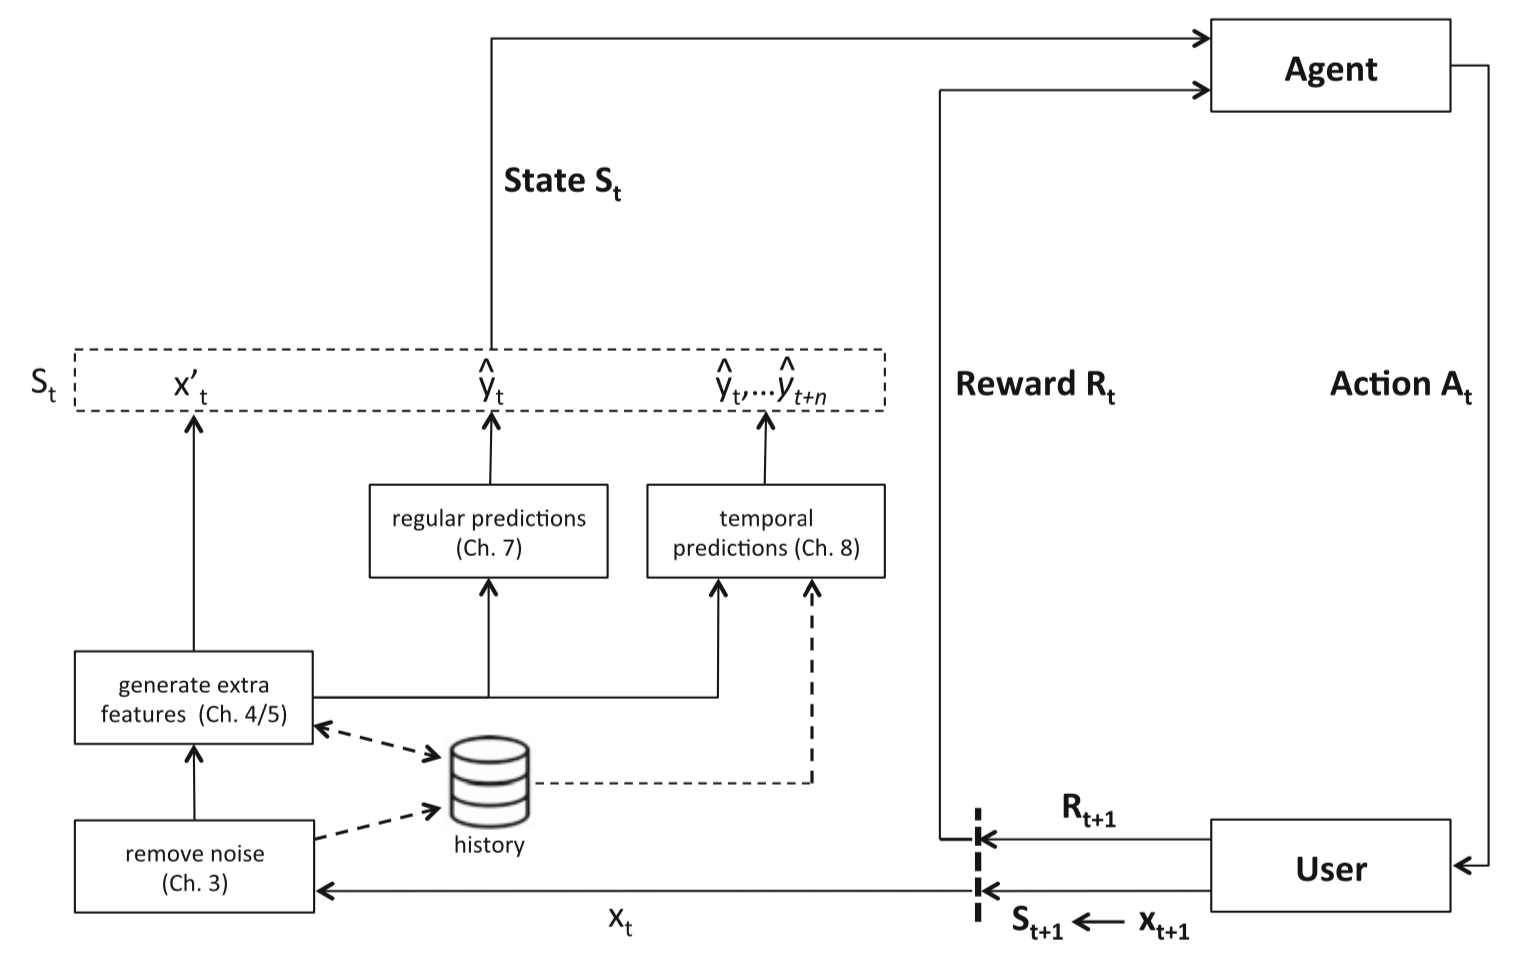
\includegraphics[width=0.5\textwidth]{figures/chapter_9_RL_loop.png}
		\caption{Reinforcement Learning in the loop for ML4QS}
		\label{fig:chapter_9_RL_loop}
	\end{figure}
	\item \textbf{Markov Property}: $\mathbb{P}\left\{R_{t+1}=r, S_{t+1}=s|S_0, A_0, R_0, ..., S_t, A_t, R_t\right\} = \mathbb{P}\left\{R_{t+1}=r, S_{t+1}=s|S_t, A_t\right\}$\\
	The conditional probabilities of future state and rewards solely depend on the last state $S_t, A_t$. 
	\item For every problem that satisfies this property, we can easily create a Markov Decision Process with a finite set of states as in Figure~\ref{fig:chapter_9_MDP}
	\begin{figure}[ht!]
		\centering
		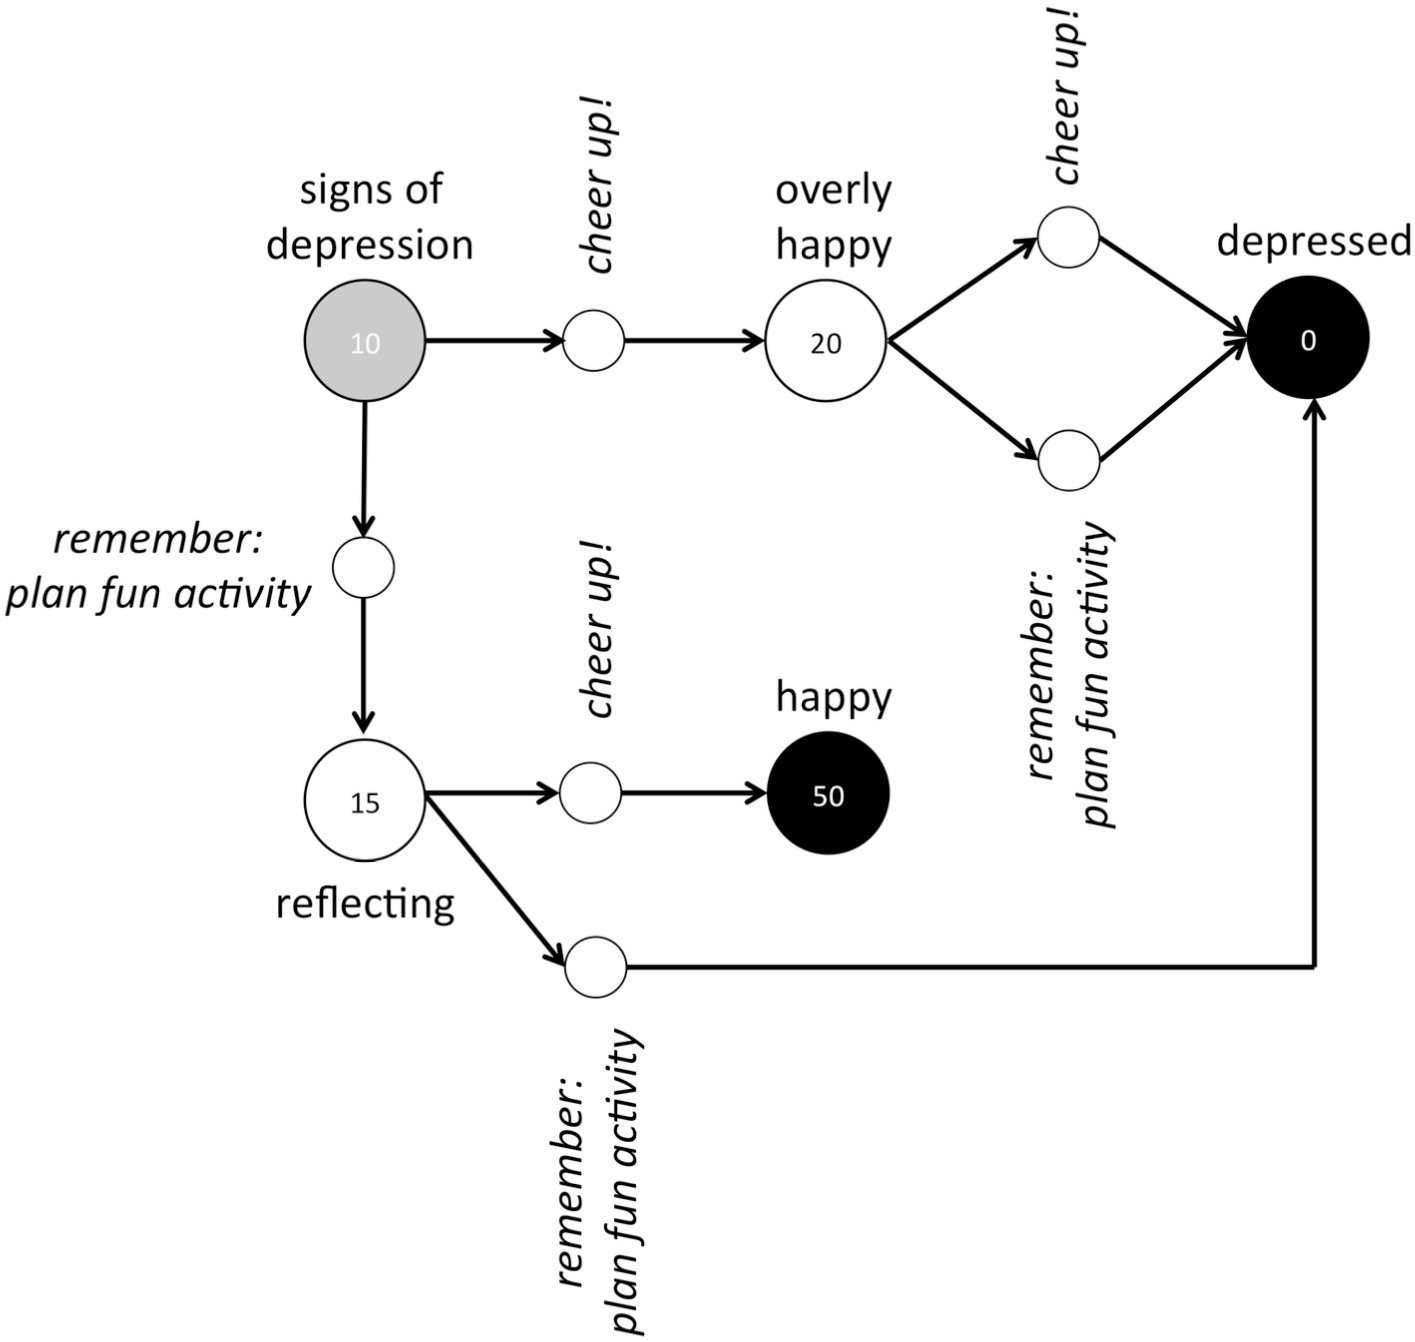
\includegraphics[width=0.35\textwidth]{figures/chapter_9_MDP.png}
		\caption{Markov Decision Process for simple example}
		\label{fig:chapter_9_MDP}
	\end{figure}
	\item \textbf{SARSA}:
	\begin{itemize}
		\item On-policy optimization, update $Q$-values by:
		$$Q(S_t, A_t) \leftarrow Q(S_t, A_t) + \alpha(R_{t+1} + \gamma Q(S_{t+1}, A_{t+1}) - Q(S_t, A_t))$$
		\item Popular policies are $\epsilon$-greedy or softmax over q-values for different actions
	\end{itemize}
	\item \textbf{Q-Learning}:
	\begin{itemize}
		\item Off-policy optimization, update by taking the maximum Q-value over next state:
		$$Q(S_t, A_t) \leftarrow Q(S_t, A_t) + \alpha(R_{t+1} + \gamma \max\limits_{A'(S_{t+1})} Q(S_{t+1}, A') - Q(S_t, A_t))$$
	\end{itemize}
	\item \textbf{Eligibility traces}: update frequently seen states in a single run more
	\begin{itemize}
		\item If we have seen a state and action combination more frequently in our history, then we want to increase the weight of the update because it is more eligible (i.e. more responsible for the outcome). We can determine the eligibility by:
		$$Z_t(s, a) = \begin{cases}
		\gamma \lambda Z_{t-1} + 1 & \text{if } s=S_t\wedge a=A_t\\
		 \gamma \lambda Z_{t-1} & \text{otherwise}
		\end{cases}$$
		\item In our learning algorithms, we can incorporate this by increasing the weight of the update, as e.g. in Q-Learning:
		$$Q(S_t, A_t) \leftarrow Q(S_t, A_t) + \alpha(R_{t+1} + \gamma \max\limits_{A'(S_{t+1})} Q(S_{t+1}, A') - Q(S_t, A_t))\cdot Z_t(s,a)$$
	\end{itemize}
	\item Usually, the Q-values are stored in a table. If the number of states and actions are very large, this is not feasible. Alternative is to learn a function/model, that takes as input the state and action, and predicts the Q-value.
	\item For continuous state spaces, we can discretize it by e.g. the \textbf{U-tree} algorithm
	\begin{itemize}
		\item Start with a single unit/leaf/discrete state where all continuous states are mapped to 
		\item Collect data by trial and error for a while and estimate the Q-values
		\item On the collected data for each leaf, we test whether we can find splits for any attribute $X_i$ with a significant difference in Q-values
		\item Choose $X_i$ and its split with the lowest $p$-value, and create new leafs. Continue until maximum number of leafs is reached
	\end{itemize}
\end{itemize}
%\appendix
%\newpage
%\input{ml4qs_appendix.tex}

\end{document}